\documentclass{sig-alternate}
\usepackage[english]{babel}
\usepackage{float}
\usepackage{graphicx}
\usepackage{xcolor}
\usepackage{minted}
\usemintedstyle{autumn}
\bibliographystyle{abbrv}

\begin{document}

\setcopyright{rightsretained}
\doi{}
\isbn{}
\conferenceinfo{ELS'17}{April 3--4, 2017, Brussel, Belgium}

\begin{CCSXML}
  <ccs2012>
  <concept>
  <concept_id>10011007.10011006.10011066</concept_id>
  <concept_desc>Software and its engineering~Development frameworks and environments</concept_desc>
  <concept_significance>500</concept_significance>
  </concept>
  <concept>
  <concept_id>10002951.10003260.10003282</concept_id>
  <concept_desc>Information systems~Web applications</concept_desc>
  <concept_significance>300</concept_significance>
  </concept>
  </ccs2012>
\end{CCSXML}

\ccsdesc[500]{Software and its engineering~Development frameworks and environments}
\ccsdesc[300]{Information systems~Web applications}

\title{Radiance - A Web Application Environment}

\numberofauthors{1}
\author{
\alignauthor
Nicolas Hafner\\
       \affaddr{ETH Zürich}\\
       \affaddr{Nürenbergstr. 17B}\\
       \affaddr{8037 Zürich, Switzerland}\\
       \email{shinmera@tymoon.eu}
}
\date{15 November 2016}

\maketitle

\begin{abstract}
  Radiance\cite{radiance} is a set of libraries that together provide an environment for web applications. Unlike traditional web frameworks that focus on a set of tools to support the construction and maintenance of a single application, Radiance attempts to allow you to run as many differing applications as desired in the same environment. This has many advantages, as frequently there are common resources in applications that should be shared between them, but cannot because the applications are separated and developed without regard for sharing. In order to fix this, Radiance provides an extensible interface mechanism to standardise the interaction between users of common resources. To facilitate the separation and encapsulation of the shared URL address space between applications, Radiance also provides a flexible routing mechanism. This mechanism is powerful enough to ensure that any application written with Radiance can be deployed on any server setup, no matter how complicated the constraints, without needing to change the source code of the application.
\end{abstract}

\printccsdesc

\keywords{Common Lisp, web framework, web development, encapsulation, interfacing}

\newpage
\section{Introduction}
While writing a website or web application is not a very complex or complicated process, doing so still usually involves performing very similar tasks every time. This lead to the rise of web frameworks-- collections of tools and libraries to take care of the most common of aspects for you. \\

A web application framework is comprised of several components. This can go from the absolute minimum of an HTTP server and URL dispatch mechanism as seen in microframeworks\cite{microframeworks}, to a vast range of tools including database access, authentication, user management, validation, API endpoints, etc. All of the components exist with the aim of reducing the amount of work necessary to write a specific web application. \\

Often these frameworks do not address questions about deployment and server setup. The assumption is made that the application will be deployed in such a fashion that it is run on a single public-facing domain, which it has complete control over. More specifically, it is assumed that the full path of the URL can be controlled. This leads to complications when multiple applications should be run on the same server. Sharing can be accomplished by using different ports for each application's server, and then using a proxying server that defers requests to the appropriate application depending on the subdomain of the request. \\

However, this does not account for all possible setups. For example, if you cannot add subdomains and would prefer to run the applications under different path prefixes, it will frequently not be possible to run the application properly. While URL rewriting by the proxying server can be used to at least get the application to dispatch, the HTTP documents returned by it will contain links that are not properly resolved and will point to invalid resources. \\

This leads to a divide in application design. If you set out to write an application that others should be able to use on their own setup, then it needs to be written in a particular way in order to account for the aforementioned setup differences. The framework will usually not help you with this in any way. \\

The problems for administrators that stem from these single-application focused frameworks do not end there, however. Many applications will need access to the same kinds of resources. Frequently, information about users, authorisation, sessions, and so forth should be shared, but cannot, because the various applications were designed individually without any concern for a standardised access or even representation of such resources. As such, running multiple applications results in duplication of information, which can be especially cumbersome for the users, as they need to track multiple registrations, logins, and so forth despite being on the same service. \\

\section{Radiance's Approach}
Radiance was designed with a different perspective in mind. Instead of viewing the application design process from the lens of the developer, it instead looks at it from the view of an administrator that would like to run an application written with Radiance on one of his servers. Doing so allowed it to come up with solutions to these problems that can simultaneously account for the needs of an administrator and those of a developer. \\

\subsection{Interfaces}
The first piece is an interface system. This system allows the specification of signatures of a package, meaning that functions, macros, variables, etc. are defined in their signature only without any actual functionality being implemented that makes them work. For example, a simplified interface to a database might look like this:

\begin{minted}[fontsize=\small]{common-lisp}
(define-interface database
  (defun select (table where &key limit skip sort))
  (defun insert (table data))
  (defun delete (table where &key limit skip sort))
  (defun update (table data where &key limit skip sort))
  (defmacro with-transaction ((name) &body body)))
\end{minted}

While the example here only shows the definition of functions and a macro, it is possible to extend the system to any definition facility desired. The description of the general behaviour of each of these definitions cannot be expressed in code however, and must thus be specified in documentation. \\

Applications can now make use of this interface and write code against it. As long as the use corresponds with the specified signatures and behaviour, the code is promised to work correctly. \\

The actual behaviour of the individual definitions is left up to an implementation of the respective interface. Such an implementation can be a regular system that simply redefines the stubs defined by the interface to do what it is supposed to. In the case of our proposed database interface, we could have multiple implementations for it, each of which connects to a particular type of database system. The choice of implementation for an interface is left up to the administrator of a Radiance installation. Since the applications that make use of an interface and the implementation for it must conform to its specified behaviour, all applications should work regardless of the particular implementation chosen. \\

Radiance provides standard interface definitions for most of the common aspects of web application programming. This allows the sharing of the previously discussed common resources such as sessions, authentication, users, profile data, and so forth. However, it is also sensible to define interfaces for commonly needed tools that may be solved in different manners. An example for this would be a caching system; the exact behaviour of the cache can vary --be it database-backed, file-backed, memory-backed, etc.-- but the usage of the system is the same regardless of implementation details. \\

In specific, Radiance defines standard interfaces for banning, rate-limiting, an administration panel, caching, authentication, sessions, users, user profiles, the HTTP server, logging, database interaction, and database record abstraction. While the interface definitions will always be around, not every interface must load an implementation unless there is an application that specifically needs it. Thus, the amount of functionality Radiance provides is also dynamic and without penalty for minimal setups. \\

Since the implementation mechanism used is a direct replacement of the interface stubs, rather than relying on some sort of indirection facility, interface functionality incurs zero overhead as well, allowing implementations to be as efficient as possible if the need arises. \\

Thus the interface mechanism solves the problem of shared access across applications without constraining the system to a particular implementation, allowing the administrator of the system to choose the appropriate implementation after the fact. \\

\subsection{Routing}
The second piece is a powerful routing system. While most frameworks seem to conflate routing and dispatching, Radiance makes a clear distinction. Dispatching is the process of determining which function to use to provide the response to a request to a particular URL. Routing is the process of transforming a URL into another. \\

The routing system lies between the HTTP server and the web applications. This leads to the following request lifecycle for a typical Radiance setup: \\

\begin{figure}[H]
  \centering
  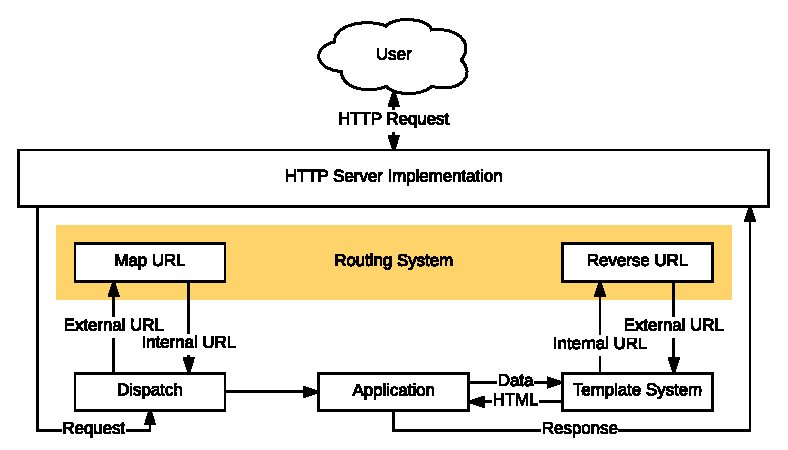
\includegraphics[width=0.42\textwidth]{request.pdf}
  \caption{Radiance Request Lifecycle}
\end{figure}

The URL on which the request arrives is transformed into an internal representation by mapping routes. This internal representation, called a ``URI'', is composed of a list of subdomains, an optional port, and a path string. The top-level domain of the request --the part of the domain we cannot change-- is stripped away. Then the request is dispatched to the first handler that matches the URI. It can then decide what to do with it, which usually is rendering some kind of template. In order to ensure that links and references within the emitted HTML can actually be resolved, the template system must use URIs that are then translated by reversal routes to produce a URL. The compelted HTML document is then sent back as a response to the request. \\

The routing system is thus responsible for maintaining the separation of the system into two different worlds: an external one that the server and users of the site interact with, and an internal one that applications deal with. \\

As an example, let us imagine a server set up on \\ \texttt{radiance.example.com/test/} that runs a single application. The application will be called ``hello'' and has the following code to define a page:

\begin{minted}{common-lisp}
(define-page index "hello/index" ()
  (r-clip:process (@template "index.ctml")))
\end{minted}

If an (untranslated) request to \texttt{hello/index} is performed, the above code will be executed, and the template system Clip\cite{clip} will render the \texttt{index.ctml} file. The template might look as follows:

\begin{minted}{html}
<link rel="stylesheet" type="text/css"
      @href="hello/static/hello/index.css" />
<h1>Hello!</h1>
\end{minted}

Clip will recognise the \texttt{@href} attribute, parse its value as a URI, send it through the reversal routes, and set the resulting URL as the value for the \texttt{href} attribute. Thus the cycle illustrated in Figure 1 is followed by our minimal setup here. \\

As it stands, Radiance would translate a request to \\\texttt{http://radiance.example.com/test/index} into the URI \\\texttt{radiance/test/index}, which is not what we need if the index page should be invoked. Routes need to be set up to handle the conversion to and from the internal representation.

\begin{minted}{common-lisp}
(define-string-route index :mapping 
  "radiance/test/(.*)" "hello/\\1")
(define-string-route index :reversal
  "hello/(.*)" "radiance/test/\\1")
\end{minted}

With these routes in place, our previous example URL will be translated into \texttt{hello/index} as required. Furthermore, the requested reversal translation of the URI \\\texttt{/static/hello/index.css} will be turned into the URL \\\texttt{\small http://radiance.example.com/test/static/hello/index.css},\\ completing the cycle properly. \\

While the above routes are fairly simplistic in their behaviour, routes can be written to perform arbitrary operations, including stashing away data in the request object for later use during reversal. This allows things like the virtual subdomain route system that is included by default. This route recognises when a request is made on the path prefix \texttt{/!/subdomain/} and translates it into a request with the subdomains set to the subdomain name in the prefix and the path stripped of this prefix. It is necessary for the corresponding reversal route to know that the initial request came through this particular route in order to appropriately translate back to the prefix, as there is no indication in the actual URI that this should happen. \\

In order for everything to fit together and work with routing, applications need to abide by some conventions that Radiance postulates. The most important one is that each application gets its own subdomain, including all subdomains on the levels below it. This allows applications to assume that they have free reign over the path part of the URL. Additionally, the path prefixes \texttt{/static/} and \texttt{/api/} are reserved by Radiance on all domains, and are used to provide static files and REST api endpoints respectively. This way, routes can be written in a more generic manner to solve common problems, rather than requiring specifically tailored rules for each application. \\

Thus, providing a generic translation mechanism for URLs allows applications to be written in a way that avoids them from clashing with each other, while at the same time gaining the ability for administrators for a setup to configure the URL namespace according to their constraints and needs. \\

\subsection{Resources}
The final piece is a generic resource mechanism that allows the exchanging of information between applications, and particularly between applications and interface implementations. This is necessary because applications may need to refer to resources provided by other components in the Radiance environment. For example, the login page and mechanism is provided by the authentication interface. An application may want to present the users a link to this page, but because the location of this page is not standardised, the application has no direct way of knowing where the page would be. Instead of specifying the page location, Radiance provides a system that allows the retrieval of arbitrary resources, and specifies that the implementation must provide the resource as requested. \\

Several standard resource types are specified, though more can be defined by an application writer, for example to provide for an extension mechanism. The most important standard resource type is the \texttt{page}, which returns a URI to the requested page, if it exists. Thus, a code like the following will produce a URL to the appropriate page:

\begin{minted}{common-lisp}
(uri-to-url (resource :auth :page "login")
            :representation :external)
\end{minted}

\section{Conclusions}
By implementing the components presented in this paper, Radiance allows for an environment that can house multiple applications in the same lisp process and seamlessly handle both the sharing of common resources, and the encapsulation and separation of each application. In order to make it feasible for every application to run on any target setup, and to make it adaptable to an administrator's requirements for the public web interface, a powerful routing system is necessary that not only handles the incoming request, but also the outgoing data. \\

These components not only present advantages to the administrator of a system, but also to the developer of an application, as they simplify and streamline various parts that would otherwise be implemented ad-hoc. This makes the resulting code easier to maintain, read, and adapt for other projects.

\bibliography{paper}
\end{document}

%%% Local Variables:
%%% mode: latex
%%% TeX-command-extra-options: "-shell-escape"
%%% TeX-master: t
%%% TeX-engine: luatex
%%% End:
